\documentclass[pdf]{beamer}
\usetheme{Copenhagen}
\usepackage{multicol, latexsym, amsmath, amssymb}
\usepackage{smartdiagram}
\usepackage{subcaption}

\setbeamertemplate{navigation symbols}{}
\newcommand{\z}{\mathbf{z}}
\newcommand{\uout}{u_{out}}
\newcommand{\vout}{v_{out}}
\newcommand{\uoutdum}{u_{out}^{dum}}
\newcommand{\uinplus}{u_{in}^{+}}
\newcommand{\uinminus}{u_{in}^{-}}
\newcommand{\winl}{w_{in}^{l}}
\newcommand{\win}{w_{in}}
\newcommand{\uin}{w_{in}}
\newcommand{\vin}{v_{in}}

\DeclareMathOperator*{\plusrightarrow}{\ensuremath{\xrightarrow{+}}}
\DeclareMathOperator*{\minusrightarrow}{\ensuremath{\xrightarrow{-}}}
\DeclareMathOperator*{\plusleftarrow}{\ensuremath{\xleftarrow{+}}}
\DeclareMathOperator*{\minusleftarrow}{\ensuremath{\xleftarrow{-}}}

\title{Updating ML Models}

\author[Ananth Mahadevan]{Ananth Mahadevan}
\date{\today}

\begin{document}
\begin{frame}
    \titlepage
\end{frame}

\begin{frame}
    \frametitle{Overview}
    \tableofcontents
\end{frame}

\section{Motivation}

\section{Problem Overview}

\section{Approaches}
\begin{frame}
  \frametitle{}
  \myNset[6]
  \smartart
\end{frame}

\begin{frame}
  \frametitle{Common Terminology}
  \begin{itemize}
    \item Fixed training Dataset $\dataset$
    \item Learning Algorithm $\alg$ (can be randomized)
    \item Datapoints to be remove $\removed$, where $|\removed|=r$, remaining dataset $\datasetprime=\dataset - \removed$
    \item Naive approach is retraining from scratch, i.e, $\alg(\datasetprime)$
    \item Mechanism $\mech$ which offers an efficient way to update the model
  \end{itemize}
\end{frame}

\subsection{Differential Privacy}
\begin{frame}
  \myNset[1]
  \smartart
\end{frame}

\begin{frame}
  \frametitle{Certified Data Removal \cite{guoCertifiedDataRemoval2020}}
  \begin{itemize}
    \item $\alg$ outputs a model in hypothesis space $\hypothesis$
    \item Defines $\epsilon$-\textit{certified removal}, $\forall \subhypothesis \subseteq \hypothesis$
    \[
      e^{-\epsilon} \le \frac{P(M(\alg(\dataset),\removed)\in \subhypothesis)}{P(A(\datasetprime)\in \subhypothesis)} \le e^{\epsilon}
    \]
    \item Insufficiency of Parametric indistinguishability
    \begin{itemize}
      \item Approximate removal processes leaves a gradient residual 
      \item Residuals can reveal the prior presence of that training sample
    \end{itemize}
  \end{itemize}
\end{frame}

\begin{frame}
  \frametitle{Removal Mechanism for Linear Classfiers}
  \begin{itemize}
    \item $\alg$ empirical risk $\risk(\w;\dataset)$ with a convex loss function $\loss(\w^{T}\x,y)$
    \item $\wopt = \alg(\dataset)=\argmin_{w}\risk(\w;\dataset)$
    \item To remove a single point $\removed = \{(\x_{n},y_{n})\}$ 
    \item Newton Update Step: $\wminus=\mech(\wopt,(\x_{n},y_{n})) = \wopt - H^{-1}_{\wopt}\nabla$
    \item Where $H_{\wopt} = \nabla^{2}\risk(\wopt,\datasetprime)$ and $\nabla = \lambda\wopt + \nabla\loss((\wopt)^{T}\x_{n},y_{n})$
    \item $H ^{-1}_{\wopt}\nabla$ is from \textit{influence function} literature 
  \end{itemize}

\end{frame}

\begin{frame}
  \frametitle{Influence Function}
  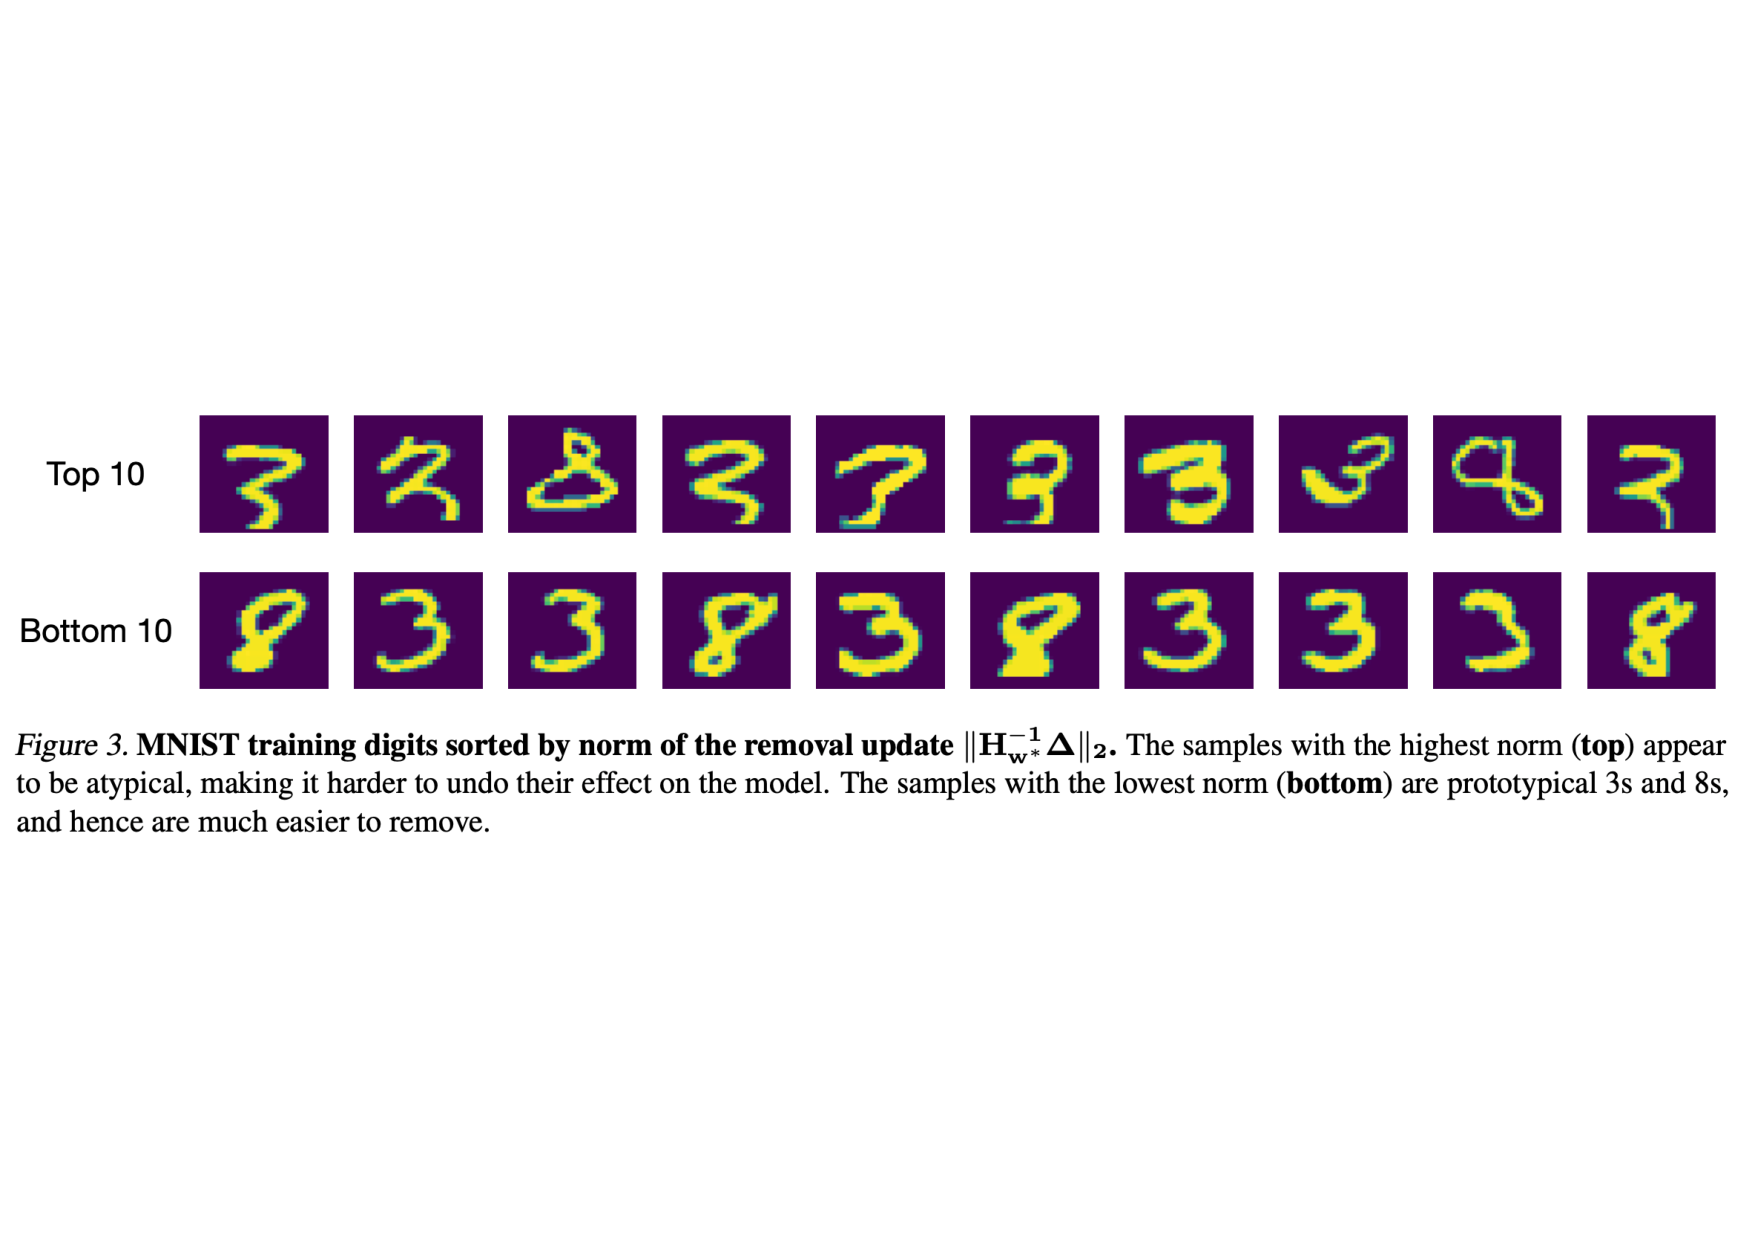
\includegraphics[width=\textwidth]{images/influence functions.pdf}
\end{frame}

\begin{frame}
  \frametitle{Certifing Removal}
  \begin{itemize}
    \item $\wminus$ is approximate close to minimizer of $\risk(\w;\datasetprime)$
    \item $\nabla\risk(\wminus;\datasetprime)$ is gradient residual and if non-zero, reveals Information
    \item Even a small $\|\nabla\risk(\wminus;\datasetprime)\|_{2}$ doesn't guarantee certifiable removal 
    \item Therefore, perturb loss at training time 
    \[
      \risk_{b}(\w;\dataset) = \sum_{i=1}^{n}\loss(\w^{T}\x_{i},y_{i})+\frac{\lambda n}{2}\|\w\|_{2}^{2} + \textbf{b}^{T}\w
    \]
    Where $\textbf{b}\in \mathbb{R}^{d}$ drawn randomly from some distribution
  \end{itemize}

\end{frame}

\subsection{Optimization}
\begin{frame}
  \myNset[2]
  \smartart
\end{frame}

\begin{frame}
  \frametitle{
    DeltaGrad \cite{wuDeltaGradRapidRetraining2020}
    }
  \begin{itemize}
    \item 
  \end{itemize}
\end{frame}


\subsection{Database Based}
\begin{frame}
  \myNset[3]
  \smartart
\end{frame}


\begin{frame}
  \frametitle{
    PrIU \cite{wuPrIUProvenanceBasedApproach2020}
    }
  \begin{itemize}
    \item 
  \end{itemize}
\end{frame}

\subsection{Information Theory}
\begin{frame}
  \myNset[4]
  \smartart
\end{frame}

\begin{frame}
  \frametitle{
    Eternal Sunshine of the Spotless Net \cite{golatkarEternalSunshineSpotless2020}
    }
  \begin{itemize}
    \item 
  \end{itemize}
\end{frame}

\subsection{Novel Pipelines}
\begin{frame}
  \myNset[5]
  \smartart
\end{frame}


\begin{frame}
  \frametitle{
    Machine Unlearning: SISA \cite{bourtouleMachineUnlearning2020}
    }
  \begin{itemize}
    \item 
  \end{itemize}
\end{frame}

\section{Next Directions}



\begin{frame}[allowframebreaks]
  \frametitle{References}
  \bibliography{UpdateMl}
  \bibliographystyle{apalike}
\end{frame}



\end{document}  